%% thesis.tex 2022/2/14
%
% Based on sample files of unknown authorship.
%
% The San Francisco State University LaTeX thesis template is
% derived from the UC Berkeley LaTeX thesis template. 
%
% The current maintainer of this work at San Francisco State University is Robert Browder.
%
% A healthy alternative to working directly in LaTeX is to use the thesisdown or bookdown package with R Studio.
% Thesis down provides the opportunity to embed executable code within the narrative flow of your document.
% Thesis down provides both PDF and HTML output.  
%
% This is the main file for this template
%
% This file is where authors may customize title, author, degree semester, degree year, degree, 
% chair, other members, and major.
%
% This file issues the commands to include each part of the document, 
% Pre-formatted parts available - abstract, preface, acknowledgments, introduction, chap1, chap2, 
% and references
% Any part can be omitted by commenting out its "include" command
% Authors may also rearrange the order of contents and add additional chapters using the mark-up examples provided


\documentclass{sfsuthesis}
\setcounter{secnumdepth}{3}
%\addbibresource{references.bib}
\usepackage[table,xcdraw]{xcolor}
% Use the graphix package with dvipdfmx when exporting to HTML to preserve figure dimensions for JPG and PNG file types. 
% For this to work you must first create an .xbb file for each file using the following command from the CLI
% ebb -x Picture2.jpg
% \usepackage[dvipdfmx]{graphicx}

% Use the graphix package without dvipdfmx when exporting to PDF
\usepackage{graphicx}

\usepackage{amsmath}
\usepackage{multirow}
\usepackage{rotating} % provides sidewaystable and sidewaysfigure


% To compile this file from the command line, run "latex thesis", then "biber thesis"
% (or "bibtex thesis", if the output from latex asks for that instead),
% and then "latex thesis" (without the quotes in each case).
%
% Alternatively, use Overleaf, MacTeX, or MikTeX to compile to PDF.
%
% To compile this file to HTML from the command line, run 
%  make4ht -f html5+mjcli thesis.tex "mathjax"
% this step requires Nodes.js, MathJax, and mjcli.js to be installed and working on your machine


% comment out the following two lines for single spacing
\def\dsp{\def\baselinestretch{2.0}\large\normalsize}
\dsp

% comment out the following line to control indentation of the first paragraph of a section
\usepackage{indentfirst}
\usepackage{appendix}
\usepackage{blindtext}
\usepackage{hyperref}

\addtolength{\abovecaptionskip}{\baselineskip}

\newtheorem{theorem}{Sample Text}

\hyphenation{mar-gin-al-ia}
\hyphenation{bra-va-do}

%path to the folder which contains figures
\usepackage{float}
\usepackage{amsmath}
\usepackage{amssymb}
\usepackage{upgreek}
\usepackage{caption}
\usepackage[labelfont=bf]{caption}
\captionsetup{skip=8pt}
\graphicspath{ {./images/} }
\usepackage{subfiles} % Best loaded last in the preamble

\usepackage{biblatex}
%\bibliography{references.bib}
\addbibresource{references.bib}
\begin{document}

% Declarations for Front Matter
\title{Prioritizing TCR Repertoire Network Properties - A Novel Approach to Select Network Signatures}
\author{Shilpika Banerjee}
\degreesemester{December}
% Select one of the semesters: December, May, or August.
\degreeyear{2022}
% Enter the year in which you are submitting your thesis.
\degree{Masters of Science}
%example: Masters of Science
\chair{Dr. Tao He}
\chairdegree{Ph.D}
\chairrank{Associate Professor}
\cochair{Dr. Mohammad R. Kafai}
\cochairdegree{Ph.D}
\cochairrank{Professor}
\memberthree{Dr. Alexandra Piryatinska}
\memberthreedegree{Ph.D}
\memberthreerank{Professor}
%\memberfour{Name of Member Four}
%\memberfourdegree{Ph.D}
%\memberfourrank{Associate Professor}
%\othermembers{Professor Roger Spam Associate Professor Michael Chex}
% For a co-chair who is subordinate to the \chair listed above
% \cochair{Professor Benedict Francis Pope}
% For two co-chairs of equal standing (do not use \chair with this one)
% \cochairs{Professor Richard Francis Sony}{Professor Benedict Francis Pope}
\numberofmembers{3}

\field{Statistics Data Science }
% Example: Computer Science: Software Engineering
% Designated Emphasis -- this is optional, and rare
% \emphasis{Colloidal Telemetry}
% This is optional, and rare
% \jointinstitution{University of Western Maryland}
% This is optional (default is Berkeley)
% \campus{Berkeley}

\maketitle
% Delete (or comment out) the \approvalpage line for the final version.
\copyrightpage
\approvalpage


% (This file is included by thesis.tex; you do not latex it by itself.)
\begin{abstract}

% The text of the abstract goes here.  If you need to use a \section
% command you will need to use \section*, \subsection*, etc. so that
% you don't get any numbering.  You probably won't be using any of
% these commands in the abstract anyway.

T-cells are one of the key components of the adaptive immune system. T-cell Receptors (TCR) are a group of protein complexes found on the surface of T-cells. TCRs are responsible for recognizing and binding to certain antigens found on abnormal cells or potentially harmful pathogens. Once the TCRs bind to the pathogens, the T-cells attack these cells and help the body fight infection, cancer, or other diseases. TCR repertoires, which are continually shaped throughout the lifetime of an individual in response to pathogenic exposure, can serve as a fingerprint of an individual’s current immunological profile. The similarity among TCRs sequence directly influences the antigen recognition breadth. Network analysis, which allows interrogation of sequence similarity, thereby adds an important layer of information. Due to the heterogeneous nature of TCR network properties, it is extremely difficult to perform statistical inference or machine learning directly between subjects. In this work, a novel method is proposed to prioritize the network properties that are associated with the outcome of interest, based on features extracted from heterogeneous global/local network properties. Schemes to select the top features associated and to simulate the network properties using the real data are also presented.  Extensive simulation studies and real data analysis were performed to demonstrate the proposed methods. Performance measures including F-1 score, false discovery rate, sensitivity, power, and stability were calculated for each model and are used for model comparison.

\end{abstract}

\subfile{sections/abstract}
\begin{frontmatter}

%\begin{preface}
\begin{comment} I owe it all to my supervisor Professor Reinhard Furrer for his guidance throughout this project.
His insights and intuition for numerical methods have been most memorable lessons for me.
I would also like to thank Professor Barbara König for not only giving interesting research
questions, but also for giving me such a rich lesson about animal behavior. My thanks also goes
to Dr. Julian Evans for his help with the data set and advice.
This thesis is but a culmination of my master program, and for that, I would also like to thank Dr.
Eva Furrer for all her care in ensuring that we have received the best education and experience. I
would also like to thank Professor Leonhard Held and Dr. Ulrike Held, who taught me practical
biostatistics.
Last but not least, thank you to my family for always believing in me.
Sandar Felicity Lim
November 2019
\end{comment}
\end{preface}

% You can delete the \clearpage lines if you don't want these to start on
% separate pages.


\begin{acknowledgments}
I would like to begin by thanking my supervisor Dr. Tao He, whose invaluable guidance and support helped me through each step of my thesis and taking it to completion. Thank you Dr. Tao He for being patient and always present for my questions. I am grateful to Dr. Li Zhang and her team, from UCSF (University of California San Francisco) for collaborating with us on this work. I would like to extend my deepest gratitude to the committee members, Dr. Mohammad R. Kafai and Dr. Alexandra Piryatinska for their support and valuable feedback.\par

I can never be grateful enough to my friends and family for their unwavering support and encouragement throughout my graduate program. Especially my mother, Mrs. Seema Banerjee, my husband, Dr. Aritra Sengupta, my sister, Nabanita Banerjee and my in-laws. Thank you for being there for me emotionally and intellectually as I worked through my coursework. I would like to dedicate this work to my father, Late Pronab Kumar Banerjee, who taught me to dream big and to never give up on my pursuits.\par

Finally, I would like to thank the mathematics department and the SF Build committee for the Bridge Award and the SF Build Agent of Change scholarships that allowed me to conduct my thesis.\par

This work was supported in part by the National Science Foundation (NSF DMS-2137983) and the National Institute of Health (NIH/NCI R21CA264381 and NIH/NLM R01LM013763-01A1).
\end{acknowledgments}
\subfile{sections/acknowledgments}
\pagestyle{headings}
\begin{KeepFromToc}
  \tableofcontents
\end{KeepFromToc}
%\tableofcontents
\clearpage
\listoftables
\clearpage
\listoffigures
\clearpage

\end{frontmatter}

\include{Introduction}
\subfile{sections/introduction}
\pagestyle{headings}
% (Optional) \part{First Part}

%\section{Methods}
%\label{sec:methods}
%\subfile{sections/method}
\include{Method}
\subfile{sections/method}
\pagestyle{headings}

\include{Implementation}
\subfile{sections/implementation}
\pagestyle{headings}
% (This file is included by thesis.tex; you do not latex it by itself.)
\chapter{Simulation Study}
\section{Data Simulation Scheme}\label{sec:sim_scheme}
Simulating network data to assess the different variable selection methods and to reproduce the experiments is vital. Data can be synthetically generated using various network simulation software tools which may require GPUs to perform large-scale simulations faster and to gain deeper insights. We present an alternative technique for simulating the TCR network data and then compute performance measures to assess the robustness, accuracy, and other parameters of the variable selection models implemented earlier. We analyze each of the network properties from the observed data, try to find any implicit relations, approximate the property distributions, and recreate the data correlation among the explanatory variables in the simulated data set. The original TCR repertoire data was heterogeneous in nature which led us to extract the summary statistics for each feature and then create an aggregated data set. Since any correlation that exists among the network features is observed in the heterogeneous (non-aggregated) form of the data, it therefore vital for us to simulate the data in the non-aggregated form and then derive the summary statistics.\par
\begin{figure}[H]
\centering
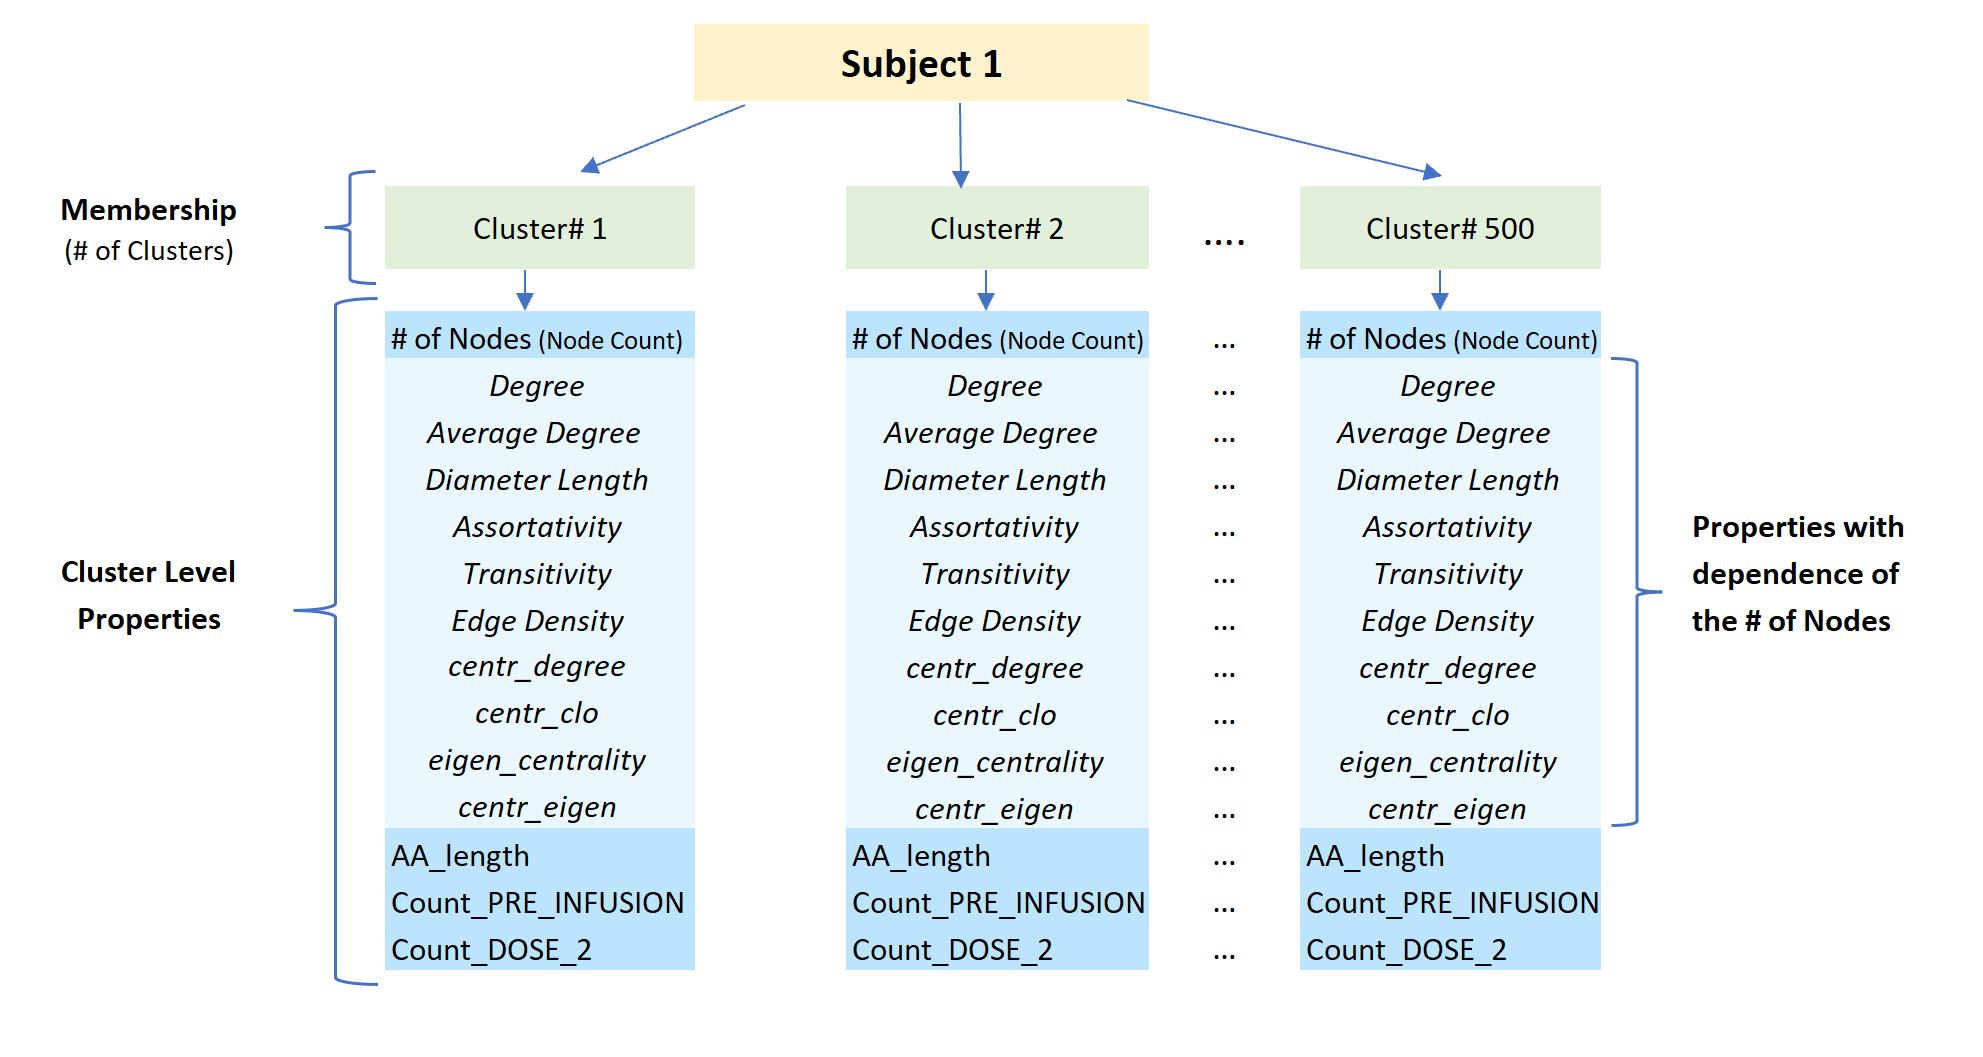
\includegraphics[scale=0.75]{Network_hierarchy.jpg}
\caption{Dependencies and Hierarchy of the Network Properties}%
{The above figure gives a general idea of how the TCR network properties are dependent on each other and a rough hierarchical structure. This information was derived by analyzing the real data.}
\label{fig:ntwrk_hier}
\end{figure}
A high-level hierarchy of the network properties as observed in the real data is shown in the \autoref{fig:ntwrk_hier}. The TCR repertoire network data of each subject has multiple clusters (membership) of varied levels of complexity. Some clusters could be dense (have more nodes), and some could be sparse (have fewer nodes). Refer \autoref{fig:cluster_ex}. Each cluster then has a varied number of nodes and associated nodal properties. As a result, simulating this network data first requires generating the clusters for a subject. Then for each cluster we simulate the \# of nodes and the associated network features.\par
\begin{figure}[H]
\centering
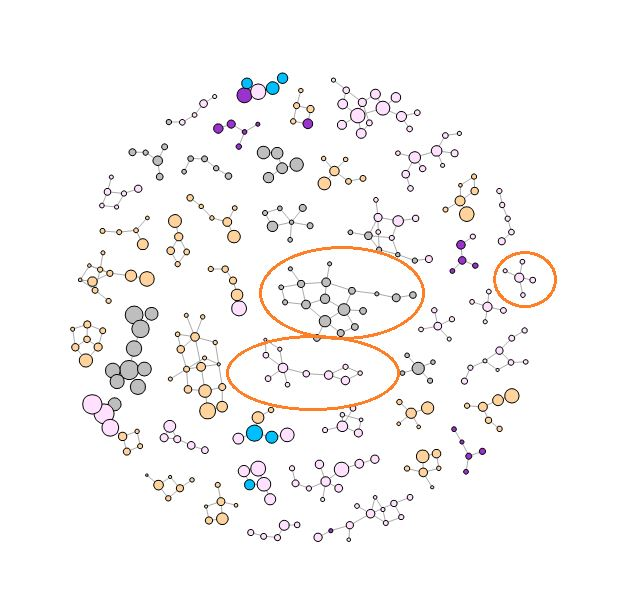
\includegraphics[scale=1]{Cluster_sample.jpg}
\caption{Sample TCR network data of a subject showing multiple clusters and nodes.}
\label{fig:cluster_ex}
\end{figure}
\subsection{Simulating Cluster-count (Membership) data}\label{subsubsec:sim_clust_cnt}
The number of clusters for each of the 65 patients were observed from the original TCR repertoire data. \autoref{fig:cluster_ex} represents the distribution of the cluster-count and the log(cluster-count) of the original TCR repertoire data. The log(cluster-count) has an approximate normal form. We then compute the mean and the standard deviation of this distribution. Using inbuilt R function, $rlnorm()$, we draw random samples from a log normal distribution, with $\text{meanlog} = \text{mean}(\log(\text{cluster-count}))$ and $\text{sdlog} = \text{sd}(\log(\text{cluster-count}))$, we generate samples which are then used as the cluster-count for 1000 dummy patients.\par
The\autoref{fig:clust_obsv_sim} represents the histogram of the cluster-count from the original observed data versus the cluster-count from the simulated data. The plots show the semblance between the original data and the simulated data. The simulated cluster-count data serves as the basis for simulating the remaining properties.\par
\begin{figure}[H]
\centering
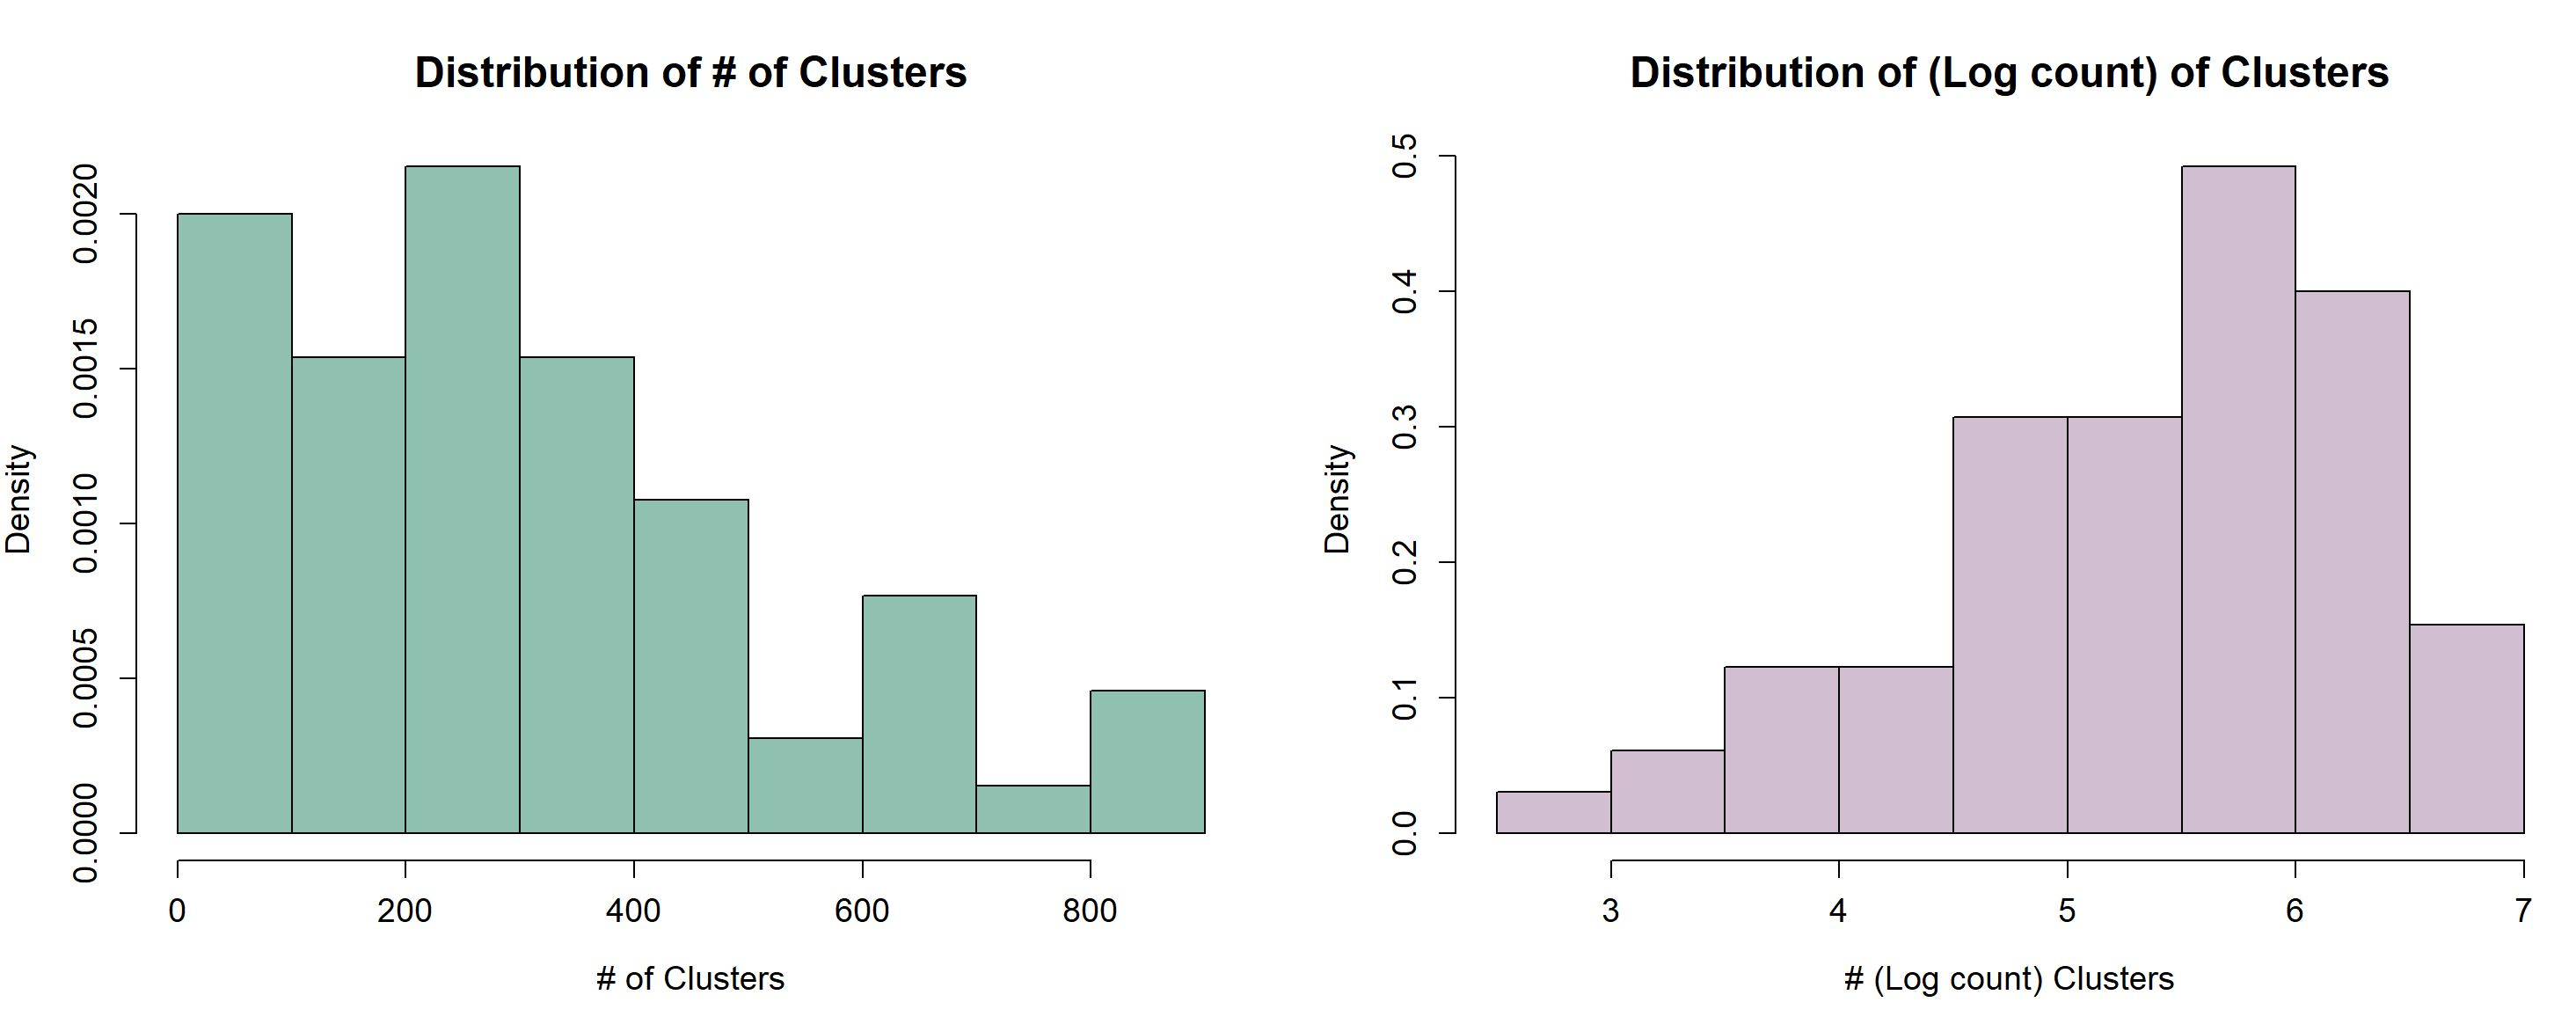
\includegraphics[scale=0.5]{Cluster_real_dt.jpg}
\caption{Histogram plot for cluster-count and log(cluster-count) of the 65 patients' TCR repertoire data.}
\label{fig:cluster_ex}
\end{figure}
\begin{figure}[H]
\centering
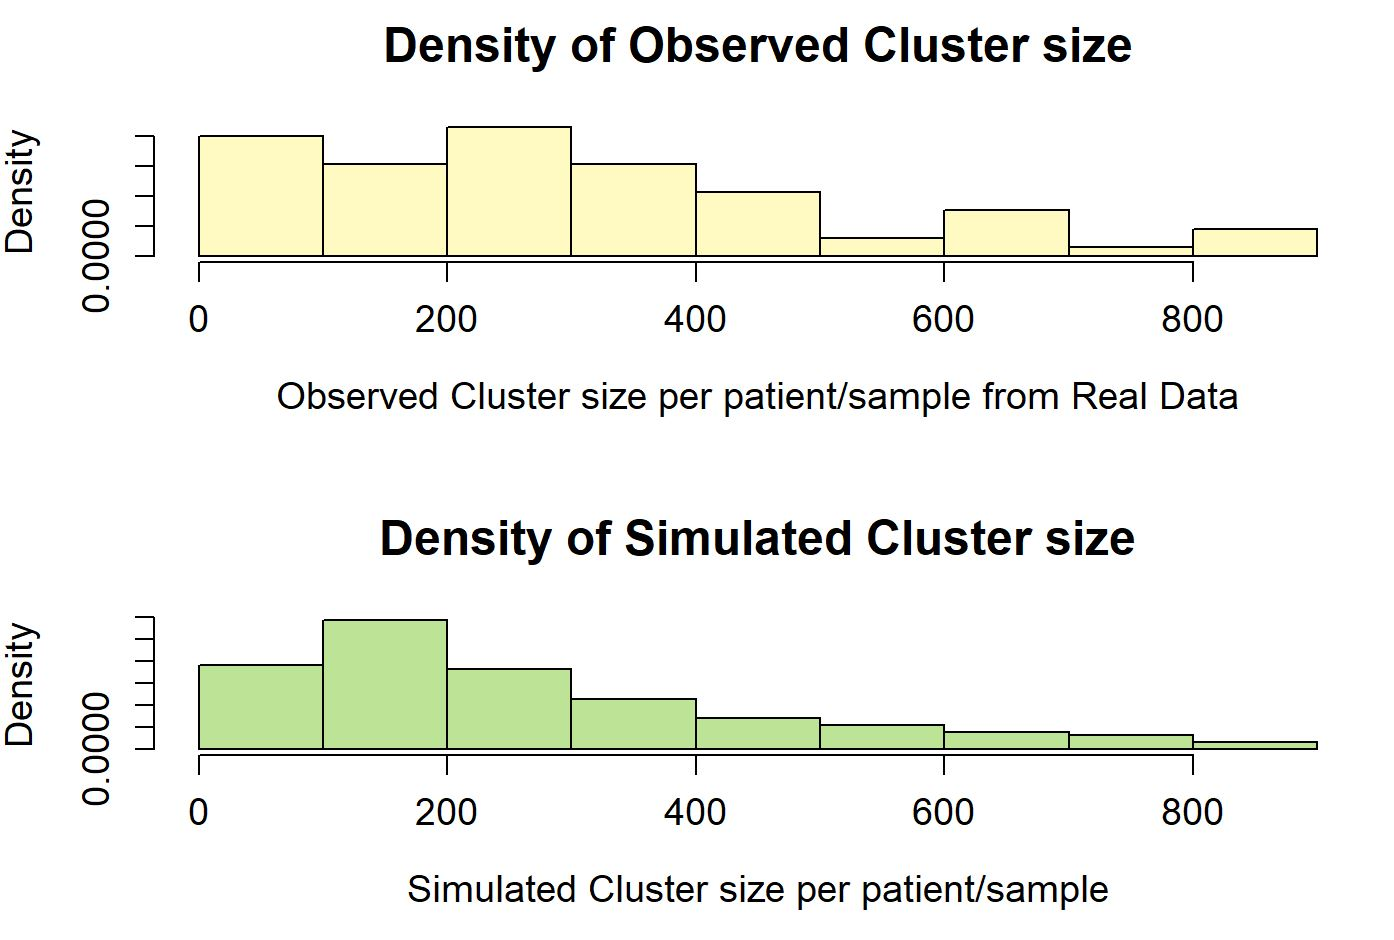
\includegraphics[scale=0.7]{Clust_obs_sim.jpg}
\caption{Histogram plots for the \lq Cluster-count' from the original data versus the \lq Cluster-count' from the simulated data.}
\label{fig:clust_obsv_sim}
\end{figure}
\subsection{Simulating Node-count data}\label{subsubsec:sim_node_cnt}
The simulated cluster-count data dictates the number of TCR network property rows that each of the 1000 dummy patients would have. We then set to simulate the node-count associated with each of the clusters. It is observed that the node-count data from the original TCR repertoire has a right-skewed distribution with maximum frequency occurring for the values 2 and 3, and the remaining subsection has an approximate log-normal form. Therefore, to simulate the node-count, the entire distribution is considered in segments. We calculated the probabilities of the node-count = 2 and 3 and simulate data for these two categories. For the remaining segment of the distribution, we draw samples from the $rlnorm()$ function using a similar technique as we did for simulating the cluster-count data. The \autoref{fig:node_count_obsv_sim} depicts the histogram of the node-count from the original observed data versus the simulated data where we can observe the similarity in the two density functions. We then derive the summary statistics for the simulated node-count data and will use the aggregated data for assessing the various models in subsequent sections.\par
\begin{figure}[H]
\centering
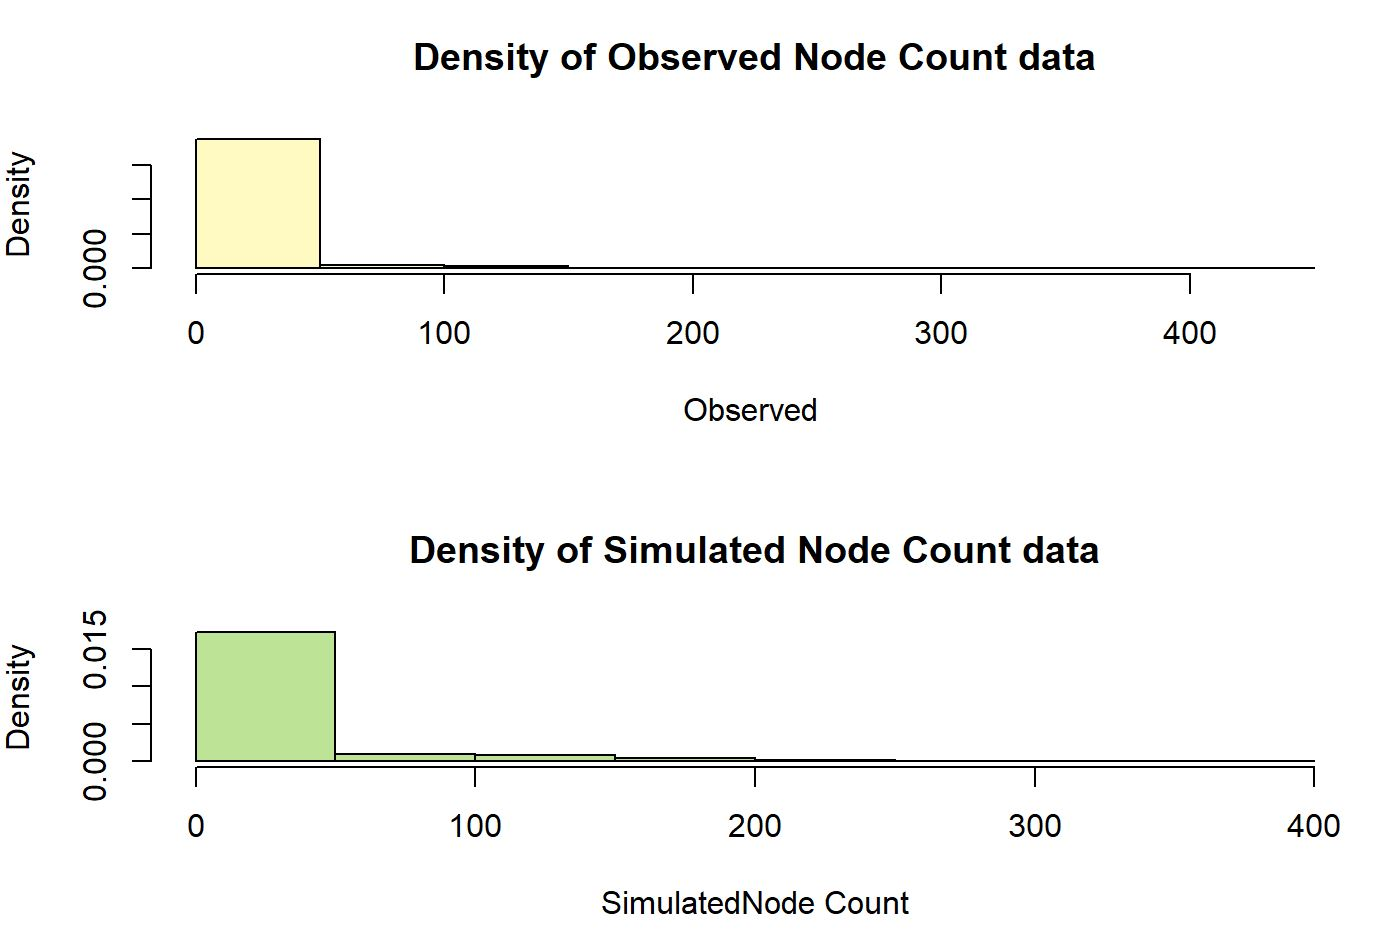
\includegraphics[scale=0.75]{Node_count_obs_sim.jpg}
\caption{Histogram plots for \lq Node-count' from the original data versus the \lq Node-count' from the simulated data.}
\label{fig:node_count_obsv_sim}
\end{figure}

\subsection{Simulating Remaining Network Properties} \label{subsubsection:sim_rem}
After the node-count data is simulated, the remaining set of network properties can be simulated. It is observed that some of the properties have a distinct value for certain values of Node-count. The \autoref{tab:node_depnd} outlines some of these relations. Probabilities of the node-count values = 2 and 3 evaluated in the \nameref{subsubsec:sim_node_cnt} sub-section are used to simulate the data for the remaining network properties. Following this, the simulated row-wise data is aggregated for each of the network properties, resulting in a single row of data per dummy patient. \autoref{fig:assort_obsv_sim} represents the histogram comparison of the observed versus simulated data of the network property called \lq Assortativity'.\par
\begin{table}[H]\centering
\caption{Dependency of some TCR properties on the Node\_count}
\begin{tabular}{|c|c|c|}\hline
\cellcolor[HTML]{D9E1F2}\textbf{TCR properties} & \cellcolor[HTML]{D9E1F2}\textbf{Values}  & \cellcolor[HTML]{D9E1F2}\textbf{Values} \\ \hline
\cellcolor[HTML]{EAEAEA}Node\_count  & \cellcolor[HTML]{EAEAEA}2 & \cellcolor[HTML]{EAEAEA}3 \\ \hline
Assortativity  & NA & -1 ($99.7\%$ times) \\ 
Transitivity  & NA & - \\ 
Degree  & 1 & - \\ 
Diam\_length  & 2 & - \\
Deg\_avg  & 1 & - \\ 
Edge\_density  & 1 & - \\ 
Centr\_degree  & 0 &  -\\ 
Centr\_clo  & NA & - \\ 
Eigen\_centrality  & 1 & - \\ 
Centr\_eigen  & NA & -\\ \hline
\end{tabular}
\label{tab:node_depnd}
\end{table}
\begin{figure}[H]
\centering
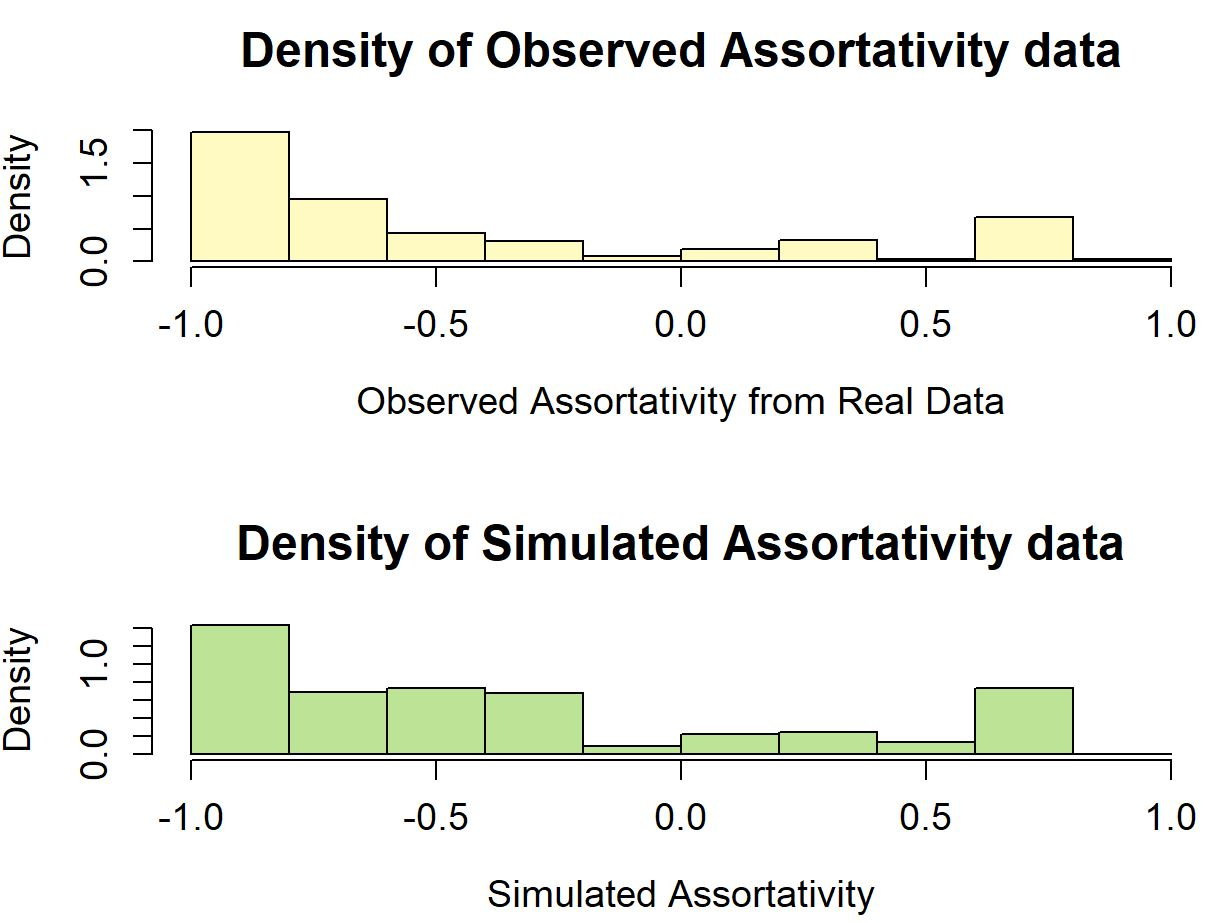
\includegraphics[scale=0.75]{Assort_obs_sim.jpg}
\caption{Histogram plots for comparing the density of \lq Assortativity' from the observed data and from the simulated data.}
\label{fig:assort_obsv_sim}
\end{figure}

\subsection{Simulating Response Variable} \label{subsubsec:simresponse}
In order to simulate the response variable, while keeping the correlation between the explanatory variables and the response intact, we use the model from the sub-section \nameref{subsec:plasso_cv}. In a binary classification setting with response variable $y_i \in{0,1}$ assume that we have independent and identically distributed observations $(\mathbf{x}_i, y_i)$ where $i=1, . . . , n$ of a $p$-dimensional vector $\mathbf{x}_i \in \mathbb{R}^p$. The log of odds is given as:
\begin{equation*}
\begin{split}
\log\{\frac{p_{\pmb{\beta}}(\mathbf{x}_i)}{1-p_{\pmb{\beta}}(\mathbf{x}_i)}\}=\beta_0+\beta_1X_1+..+\beta_pX_p=\eta_{\pmb{\beta}}(\mathbf{x}_i)
\end{split}
\end{equation*}
where $p_{\pmb{\beta}} = \mathbb{P}_{\pmb{\beta}}(y_i=1|\mathbf{x}_i)$ and $\pmb{\beta}=(\beta_0,\beta_1, .., \beta_p)^T$ are the coefficients for the $p$ predictors.\par
Using the Lasso model from \autoref{subsec:plasso_cv} where we obtained feature indexes [25, 43, 82, 89] as the significant variables. We use these as the true causal variables $X_1,...,X_4$ for simulating the response variable $y_i$'s where $i\in 1,..,1000$. The log of odds $\eta_{\pmb{\beta}}(\mathbf{x}_i)$ and $p_{\pmb{\beta}}=\mathbb{P}_{\pmb{\beta}}(y_i=1|\mathbf{x}_i)$ can be written as:
\begin{equation}\label{eq:9}
\eta_{\pmb{\beta}}(\mathbf{x}_i)=\beta_0+\beta_1X_1+..+\beta_4X_4
\end{equation}
\begin{equation}\label{eq:10}
p_{\pmb{\beta}} = \mathbb{P}_{\pmb{\beta}}(y_i=1|\mathbf{x}_i) =  \frac{\exp(\eta_{\pmb{\beta}}(\mathbf{x}_i))}{1+\exp(\eta_{\pmb{\beta}}(\mathbf{x}_i))}
\end{equation}
where the $\pmb{\beta}$ coefficients are artificially created. We then sample randomly from a Bernoulli distribution using the function $rbern()$ such that 1000 random samples are generated with probability $=p_{\pmb{\beta}}$. These random samples are then used as simulated response values for our study.\par

\section{Simulation Results}\label{sec:simresults}
The simulated network property data is aggregated to produce summary statistics for each subject and is indexed like what was done for the original data. The simulated data also consists of 89 network features (individual summary statistics) and 15 network properties (feature blocks deduced by aggregating the summary statistics). The data set is then down-sampled to accommodate for the data imbalance. We assess the Lasso\_CV, Plasso, Group Lasso\_CV, Group Plasso, and Exclusive Lasso models using the simulated data. Performance measures are computed by iteratively running the variable selection models on the simulated data.\par

\subsection{Evaluation Criteria} \label{subsec:evalcrt}
We used the following measures - Sensitivity, False Discovery Rate (FDR), F1 score, Power, and Stability to evaluate the
performances of the different variable selection models. A false-positive finding means the selection of any predictor variable except the causal variables by the feature selection method. Sensitivity is defined as the proportion of correctly identifying causal variables among all causal variables in a single iteration. FDR is defined as the frequency of false-positive findings among all variables selected per method and
iteration. F-1 score is the harmonic mean of the sensitivity and (1-FDR). It is a measure of performance accuracy of the model. The power of each causal variable is calculated as the frequency of correct selections among all iterations. To estimate stability of a variable selection model, all pairwise combinations of the selected variables list from each iteration are considered. For each pair, the stability of the two lists of selected variables is determined using the Jaccard’s index given as: $J(A_i,A_j)=\frac{|A_i\cap A_j|}{|A_i\cup A_j|}$, where $A_i$ is the list of variables selected in the $i^{\text{th}}$ iteration and $A_j$ is the list of variables selected in the $j^{\text{th}}$ iteration such that $i\ne j$ and $i,j\in 1,2,..,I (\text{ total number of iterations})$. Jaccard's index, $J(A_i,A_j)=0$ if the two lists do not overlap, and $J(A_i,A_j)=1$ if the two lists contain the same variables. The average of all pairs is used as the stability value for that method.

\subsection{Simulation Results from Group Lasso\_CV and Group Plasso} \label{subsec:simstudy_grplasso}
The assessment of the Group Lasso\_CV and the Group Plasso models on the simulated data is done using the true causal variables derived using the Lasso\_CV model (refer \autoref{subsec:plasso_cv}) on the original data, as the \lq gold-standard'. The causal network properties (feature blocks) that correspond to the top network features are derived from \autoref{subsec:plasso_cv}. The performance measures for the simulation study on Group Lasso\_CV and Group Plasso models are shown in the \autoref{tab:grp_lasso_vs_lasso_sim_study}. It is observed that both Group Lasso\_CV and Group Plasso models have high sensitivity which is desirable. The FDR value for the Group Plasso model is lower than that of the Group Lasso\_CV model which is as expected. The Group Plasso model however has a much higher stability than the Group Lasso\_CV model.\\

\begin{table}[H]
\caption{Performance measures of Group Lasso\_CV and Group Plasso models.}
\resizebox{\textwidth}{!}{%
\begin{tabular}{|c|c|c|c|c|c|c|}\hline
\cellcolor[HTML]{D9E1F2}\textbf{Models} & 
\cellcolor[HTML]{D9E1F2}\textbf{True Group Indexes}  & 
\cellcolor[HTML]{D9E1F2}\textbf{Sensitivity} & 
\cellcolor[HTML]{D9E1F2}\textbf{FDR} &
\cellcolor[HTML]{D9E1F2}\textbf{F1} &
\cellcolor[HTML]{D9E1F2}\textbf{Power} &
\cellcolor[HTML]{D9E1F2}\textbf{Stability} \\ \hline
Group Lasso\_CV & Group - 5, 8, 14, 15   & 0.775 & 0.5324 & 0.5597 & 0.8, 1.0, 0.8, 0.5 &  0.5911\\ \hline
Group Plasso & Group - 5, 8, 14, 15 & 0.7 & 0.45297 & 0.6094 & 1.0, 1.0, 0.7, 0.1 & 0.8123 \\ \hline
\end{tabular}}
\label{tab:grp_lasso_vs_lasso_sim_study}
\end{table}

\subsection{Simulation Results from Lasso\_CV and Plasso} \label{subsec:simstudy_plasso}
Consider the top network features derived from the Lasso\_CV model (refer \autoref{subsec:plasso_cv}) as the \lq gold-standard' for the causal variables. The Lasso\_CV and the Plasso models are assessed using these true causal variables. It is observed that the Plasso model outperforms the Lasso\_CV model in terms of the FDR and F1 score. The remaining performance measures are at par. Refer \autoref{tab:lasso_sim_study}.\\ 
\begin{table}[H]
\caption{Performance measures of Lasso\_CV and Plasso models.}
\resizebox{\textwidth}{!}{%
\begin{tabular}{|c|c|c|c|c|c|c|}\hline
\cellcolor[HTML]{D9E1F2}\textbf{Models} & 
\cellcolor[HTML]{D9E1F2}\textbf{True Feature Indexes}  & 
\cellcolor[HTML]{D9E1F2}\textbf{Sensitivity} & 
\cellcolor[HTML]{D9E1F2}\textbf{FDR} &
\cellcolor[HTML]{D9E1F2}\textbf{F1} &
\cellcolor[HTML]{D9E1F2}\textbf{Power} &
\cellcolor[HTML]{D9E1F2}\textbf{Stability} \\ \hline
Lasso\_CV & 25, 43, 82, 89 & 1 & 0.5065 & 0.6594 & 1.0, 1.0, 1.0, 1.0 & 0.9212 \\ \hline
Plasso &  25, 43, 82, 89 & 1 & 0.2533 & 0.8533 & 1.0, 1.0, 1.0, 1.0 & 0.9111\\ \hline
\end{tabular}}
\label{tab:lasso_sim_study}
\end{table}

\subsection{Simulation Results from Exclusive Lasso\_CV} \label{subsec:simstudy_exclusvlasso}
For assessing the Exclusive Lasso model on the simulated data we use the top network features, derived using the Lasso\_CV model (refer \autoref{subsec:plasso_cv}), as the \lq gold-standard' for the causal variables. It is observed that Exclusive Lasso consistently identifies the true causal variables in every iteration and therefore has a perfect sensitivity value. This result asserts the findings from the Lasso models. Note that Exclusive Lasso shows a very high FDR and low F1 values. This observation is due to the compulsion of the Exclusive Lasso model to select at least one feature from each of the feature blocks. \\[4pt]
\begin{table}[H]
\caption{Performance measures of Exclusive Lasso model.}
\resizebox{\textwidth}{!}{%
\begin{tabular}{|c|c|c|c|c|c|c|}\hline
\cellcolor[HTML]{D9E1F2}\textbf{Models} & 
\cellcolor[HTML]{D9E1F2}\textbf{True Feature Indexes}  & 
\cellcolor[HTML]{D9E1F2}\textbf{Sensitivity} & 
\cellcolor[HTML]{D9E1F2}\textbf{FDR} &
\cellcolor[HTML]{D9E1F2}\textbf{F1} &
\cellcolor[HTML]{D9E1F2}\textbf{Power} &
\cellcolor[HTML]{D9E1F2}\textbf{Stability} \\ \hline
Exclusive Lasso\_CV & 25, 43, 82, 89 & 1 & 0.8 & 0.3333 & 1, 1, 1, 1 & 1 \\ \hline
\end{tabular}}
\label{tab:exclusv_lasso_sim_study}
\end{table}
\subfile{sections/simulationstudy}
% (This file is included by thesis.tex; you do not latex it by itself.)
\chapter{Discussion}
All analyses and implementations were done using the R programming language with base packages and the subsequent analysis-specific packages. The code is available on \href{https://github.com/ShilpikaB/Prioritizing-Network-Properties-of-T-Cell-Receptors}{\textbf{GitHub}} for reference.
\section{Inferences from Real Data Analysis}\label{sec:realdat_ana}
This thesis focuses on the application of variable selection techniques like Lasso, Group Lasso and Exclusive Lasso using different hyperparameter tuning techniques --- cross-validation and permutation assisted tuning. Using the original sample data, the Group Lasso\_CV model was able to prioritize three of the network properties (feature blocks) --- \lq Membership' (\# of Clusters), \lq Count\_PRE\_INFUSION', and \lq Count\_DOSE\_2'. The Group Plasso model selected only two of the network properties --- \lq Membership' (\# of Clusters) and \lq Count\_PRE\_INFUSION'. The difference in the output of the two models can be attributed to the characteristics of the permutation tuning of having lower false positives (\cite{permassisttune}Yang \textit{et al.}, 2020) in comparison to the cross-validation technique. Therefore, the Group Plasso model appears to be more stringent than Group Lasso\_CV in performing variable selection on the network feature blocks. When using Lasso\_CV and Plasso both models selected the same set of network features as the top performing variables --- the \lq maximum' summary statistics for the TCR network properties \lq Count\_PRE\_INFUSION', \lq diam\_length', \lq eigen\_centrality', \lq centr\_eigen'. Exclusive Lasso (using only cross-validation) model reaffirmed the findings from Lasso\_CV and Plasso by selecting the same set of network features from their corresponding feature blocks.\par

\section{Model Performance Comparison} \label{sec:perf_measure}
From the simulation study on the Group Lasso\_CV and Group Plasso models it is observed that the Group Plasso model has a higher F1 score value. Given that the F1 score aggregates the results from the \lq Sensitivity' and the \lq FDR' values, a higher F1 score is desirable. The Group Plasso model has a stability of $\sim 81\%$ while Group Lasso\_CV has only $\sim 59\%$ stability. This shows that permutation assisted tuning improved the model stability significantly over cross-validation technique.\par
Similarly, when comparing the Lasso\_CV and the Plasso models, the latter has a much lower FDR value and hence a higher F1 score. This aligns with the advantage of permutation assisted tuning having lower false positives than cross-validation technique. Being able to lower the false positives while having the other performance measures almost similar to that of Lasso\_CV, makes the Plasso model a preferable choice for variable selection than Lasso\_CV.\par
Formally verification is required to prove whether the performance of permutation assisted tuning is superior to that of cross-validation for all variable selection problems.\par 

\section{Significant TCR Network Properties and Features} \label{sec:add_features}
Referring to the output from the \autoref{tab:grp_lasso_vs_lasso_sim_study}, the aggregated list of group indexes selected by both Group Lasso\_CV and Group Plasso models are - \lq Membership' (\# of Clusters), \lq Count\_PRE\_INFUSION', and \lq Count\_DOSE\_2'. These feature blocks correspond to the most significant TCR network properties. Similarly, using Lasso\_CV and Plasso models on the original data identify the \lq maximum' summary statistics for \lq Count\_PRE\_INFUSION', \lq diam\_length', \lq eigen\_centrality', \lq centr\_eigen' emerge as the top performing TCR network features.\par
\subfile{sections/discussion}

\printbibliography
%\bibliography{references.bib}

%\listoftables
%\clearpage
%\listoffigures
%\clearpage


\appendix
\addappheadtotoc



\section{Appendix A: List of California State University Campuses}

\begin{itemize}
\item California State University, Bakersfield
\item California State University Channel Islands
\item California State University, Chico
\item California State University, Dominguez Hills
\item California State University, East Bay
\item California State University, Fresno
\item California State University, Fullerton
\item Humboldt State University
\item California State University, Long Beach
\item California State University, Los Angeles
\item California State University Maritime Academy
\item California State University, Monterey Bay
\item California State University, Northridge
\item California State Polytechnic University, Pomona
\item California State University, Sacramento
\item California State University, San Bernardino
\item San Diego State University
\item San Francisco State University
\item San José State University
\item California Polytechnic State University, San Luis Obispo
\item California State University San Marcos
\item Sonoma State University
\item California State University, Stanislaus
\end{itemize}


\section{Appendix B: Abbreviations of California State University Campuses}

\begin{itemize}
\item CSU Bakersfield
\item CSU Channel Islands
\item Chico State
\item CSU Dominguez Hills
\item Cal State East Bay
\item Fresno State
\item Cal State Fullerton
\item Humboldt State
\item Cal State Long Beach
\item Cal State LA
\item Cal Maritime
\item CSU Monterey Bay
\item CSUN
\item Cal Poly Pomona
\item Sacramento State
\item Cal State San Bernardino
\item San Diego State
\item San Francisco State
\item San José State
\item Cal Poly San Luis Obispo
\item CSU San Marcos
\item Sonoma State
\item Stanislaus State
\end{itemize}

\begin{subappendices}
%\subsection{Sub Appendix}
\end{subappendices}


\subfile{sections/appendix}

\end{document}
